\documentclass[12pt]{beamer}

% for themes, etc.
\mode<presentation>
{ \usetheme{Copenhagen}
  \usecolortheme{seahorse}{}
  \usefonttheme{professionalfonts}
}
\setbeamertemplate{itemize items}[default]
\setbeamertemplate{enumerate items}[default]
\setbeamertemplate{navigation symbols}{}
\setbeamertemplate{headline}{}
\setbeamertemplate{footline}{}

\usepackage{times}  % fonts are up to you
\usepackage{proof}
\usepackage{listings}
\usepackage{courier}
\usepackage{graphicx}
\usepackage{stmaryrd}

\usepackage{tikz}
\newcommand*\circled[1]{\tikz[baseline=(char.base)]{
            \node[shape=circle,draw,double,inner sep=1pt] (char) {#1};}}

\DeclareMathOperator{\Wtype}{W}
\DeclareMathOperator{\Mtype}{M}
\DeclareMathAlphabet{\mathbfsf}{\encodingdefault}{\sfdefault}{sb}{n}
\def\Type{\mathbfsf{Type}}


\lstset{columns=fullflexible}
\lstset{
  literate={->}{$\to$ }{1}
           {(->)}{$(\to)$ }{1}
           {=>}{$\Rightarrow$ }{1}
           {<-:}{$\Mapsfrom$ }{1}
           {(<-:)}{($\Mapsfrom$)}{1}
           {:E}{$\in$ }{1}
           {:<}{$\subseteq$ }{1}
           {forall}{$\forall$}{1}
           {(<+>)}{($\oplus$) }{1}
           {<+>}{$\oplus$ }{1}
           {<<*>>}{$\circled{$\star$}$ }{1}
           {<<map>>}{$\circled{\$}$ }{1}
           {(<<map>>)}{($\circled{\$}$) }{1}
           {(<<*>>)}{($\circled{$\star$}$) }{1}
           {Nat}{$\mathbb{N}$}{1}
           {Int}{$\mathbb{Z}$}{1},
  escapeinside=||,
  moredelim=**[is][\color{red}]{@}{@},
}
\lstset{language=Haskell}

% these will be used later in the title page
\title{Programming in Vinyl}
\author{Jon Sterling\\
    FOBO
}

\begin{document}

% this prints title, author etc. info from above
\begin{frame}
\titlepage
\end{frame}

\section{Extensible Records and Row Polymorphism}

\begin{frame}[fragile]
  \frametitle{Records in GHC 7.8}\pause
  \begin{itemize}
    \item Haskell records are nominally typed\pause
    \item They may not share field names
  \end{itemize}
  \pause
  \begin{lstlisting}
  data R = R { x :: X } |\pause|
  data R' = R' { x :: X } -- ^ Error
  \end{lstlisting}
\end{frame}

\begin{frame}
  \frametitle{Records in GHC 7.8}
  \only<1>{Records are...}
  \only<2>{\Large\centerline{anticompositional}}
\end{frame}

\begin{frame}
  \frametitle{Structural Typing}\pause
  \begin{itemize}
    \item Sharing field names and accessors\pause
    \item Record types may be characterized \emph{extensionsionally}
  \end{itemize}
\end{frame}

\begin{frame}
  \frametitle{Row Polymorphism}\pause
  How do we express the type of a function which adds a field to a record?\pause
  \only<3>{
    \[
      \infer{ f(x) : \{foo:A, bar:B\} }{ x : \{foo:A\} }
    \]
  }
  \only<4>{
    \[
      \infer{ f(x) : \{foo:A, bar:B; \vec{rs}\} }{ x : \{foo:A; \vec{rs}\} }
    \]
  }
\end{frame}

\begin{frame}[fragile]
  \frametitle{Roll Your Own in Haskell}\pause
  \begin{lstlisting}
  data (s :: Symbol) ::: (t :: *) = Field |\pause|

  data Rec :: [*] -> * where |\pause|
    RNil :: Rec '[] |\pause|
    (:&) :: !t -> !(Rec rs) -> Rec ((s ::: t) ': rs)

  |\pause|
  class s :E (rs :: [*])|\pause|
  class ss :< (rs :: [*]) where
    cast :: Rec rs -> Rec ss|\pause|
  (=:) : s ::: t -> t -> Rec '[s ::: t]|\pause|
  (<+>) : Rec ss -> Rec ts -> Rec (ss ++ ts)
  \end{lstlisting}
\end{frame}

\begin{frame}[fragile]
  \frametitle{Roll Your Own in Haskell}\pause
  \begin{lstlisting}
  f :: "foo" ::: A :E rs => Rec rs -> Rec ("bar" ::: B ': rs)
  \end{lstlisting}
\end{frame}

\section{Universes \`a la Tarski}

\begin{frame}
  \frametitle{Universes \`a la Tarski}\pause
  \begin{itemize}
    \item A type $\mathcal{U}$ of \textbf{codes} for types.
      \pause
    \item Function $El_\mathcal{U} : \mathcal{U}\to\Type$.
      \pause
      \[
        \infer{
          \Gamma\vdash El_\mathcal{U}(s) : \Type
        }{
          \Gamma\vdash s : \mathcal{U}
        }
      \]
  \end{itemize}
\end{frame}

\begin{frame}
  \frametitle{Universes \`a la Tarski}
  \begin{center}
    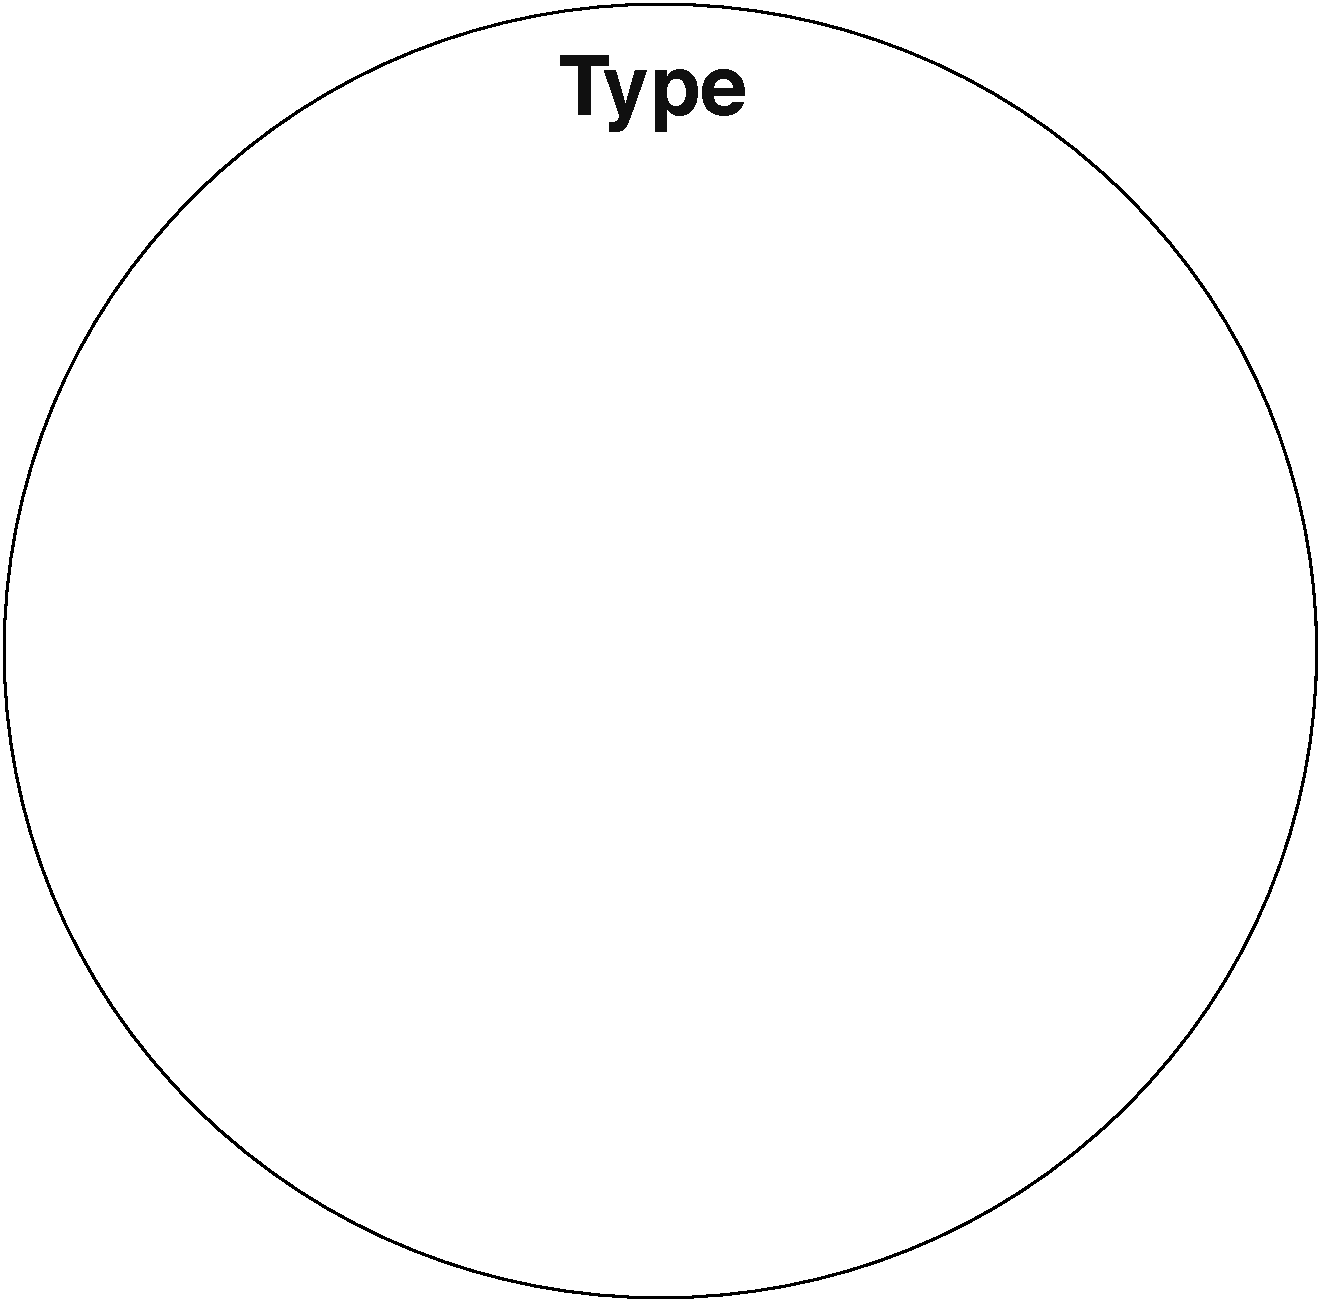
\includegraphics[width=2.8in]{universe-empty.pdf}
  \end{center}
\end{frame}

\begin{frame}
  \frametitle{Universes \`a la Tarski}
  \begin{center}
    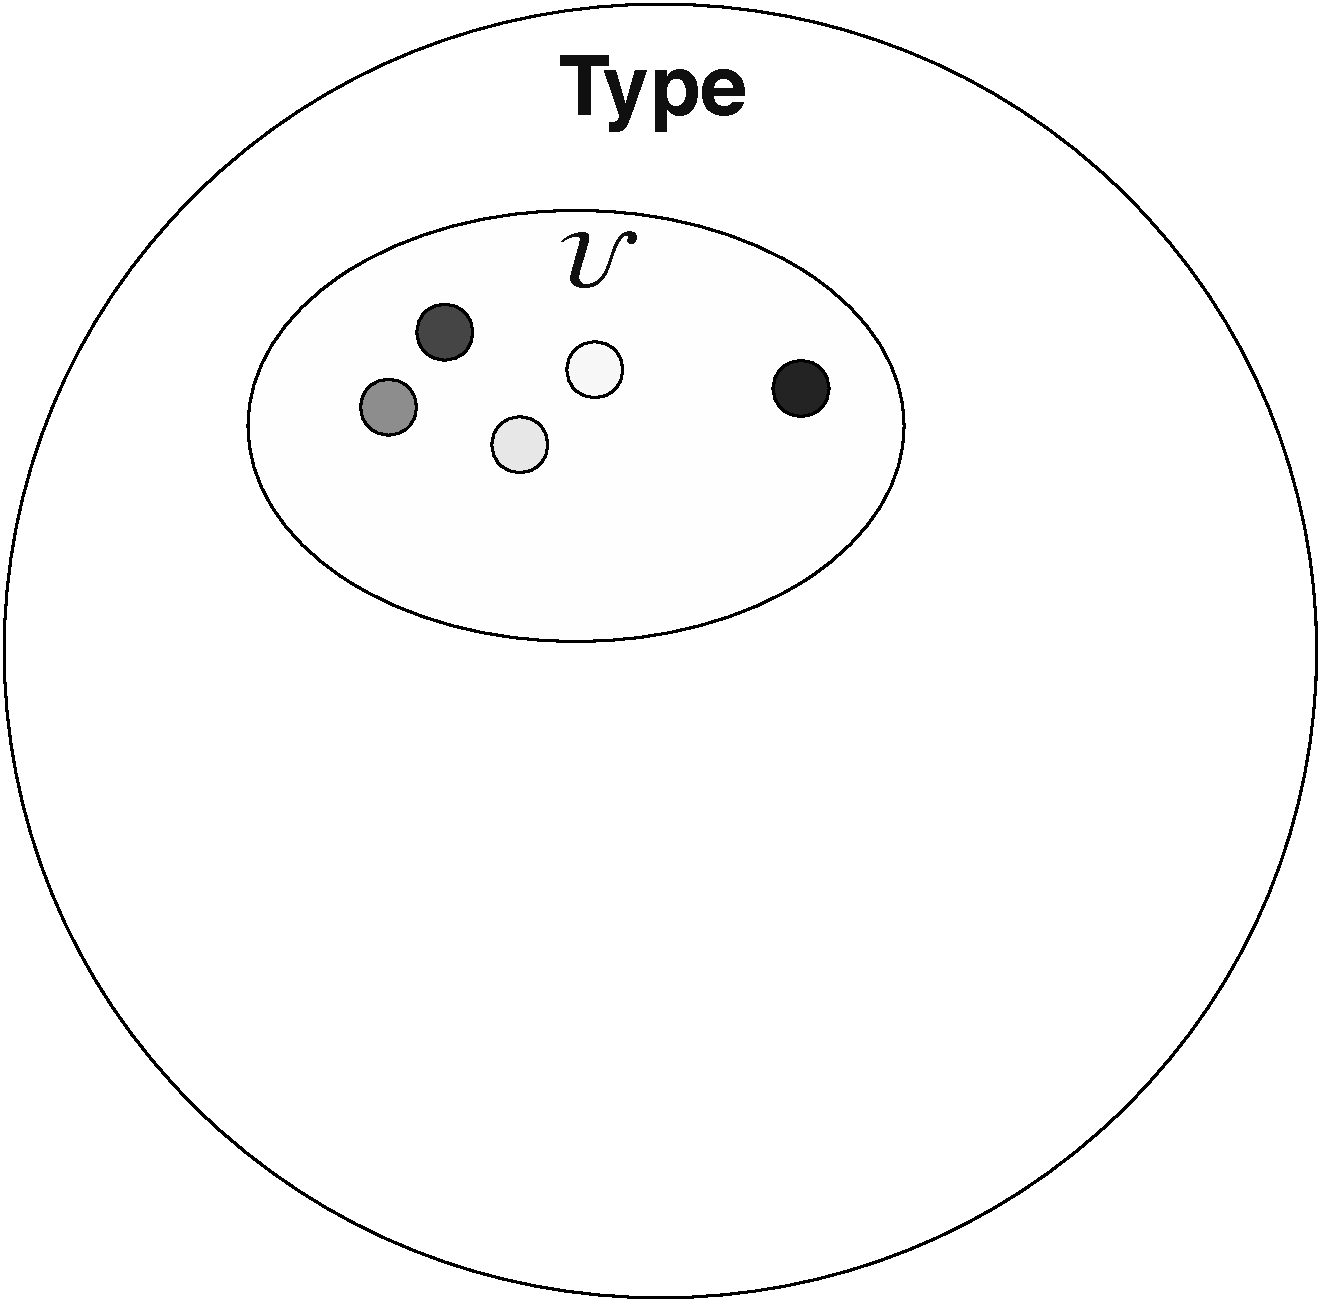
\includegraphics[width=2.8in]{universe-embedded.pdf}
  \end{center}
\end{frame}

\begin{frame}
  \frametitle{Universes \`a la Tarski}
  \begin{center}
    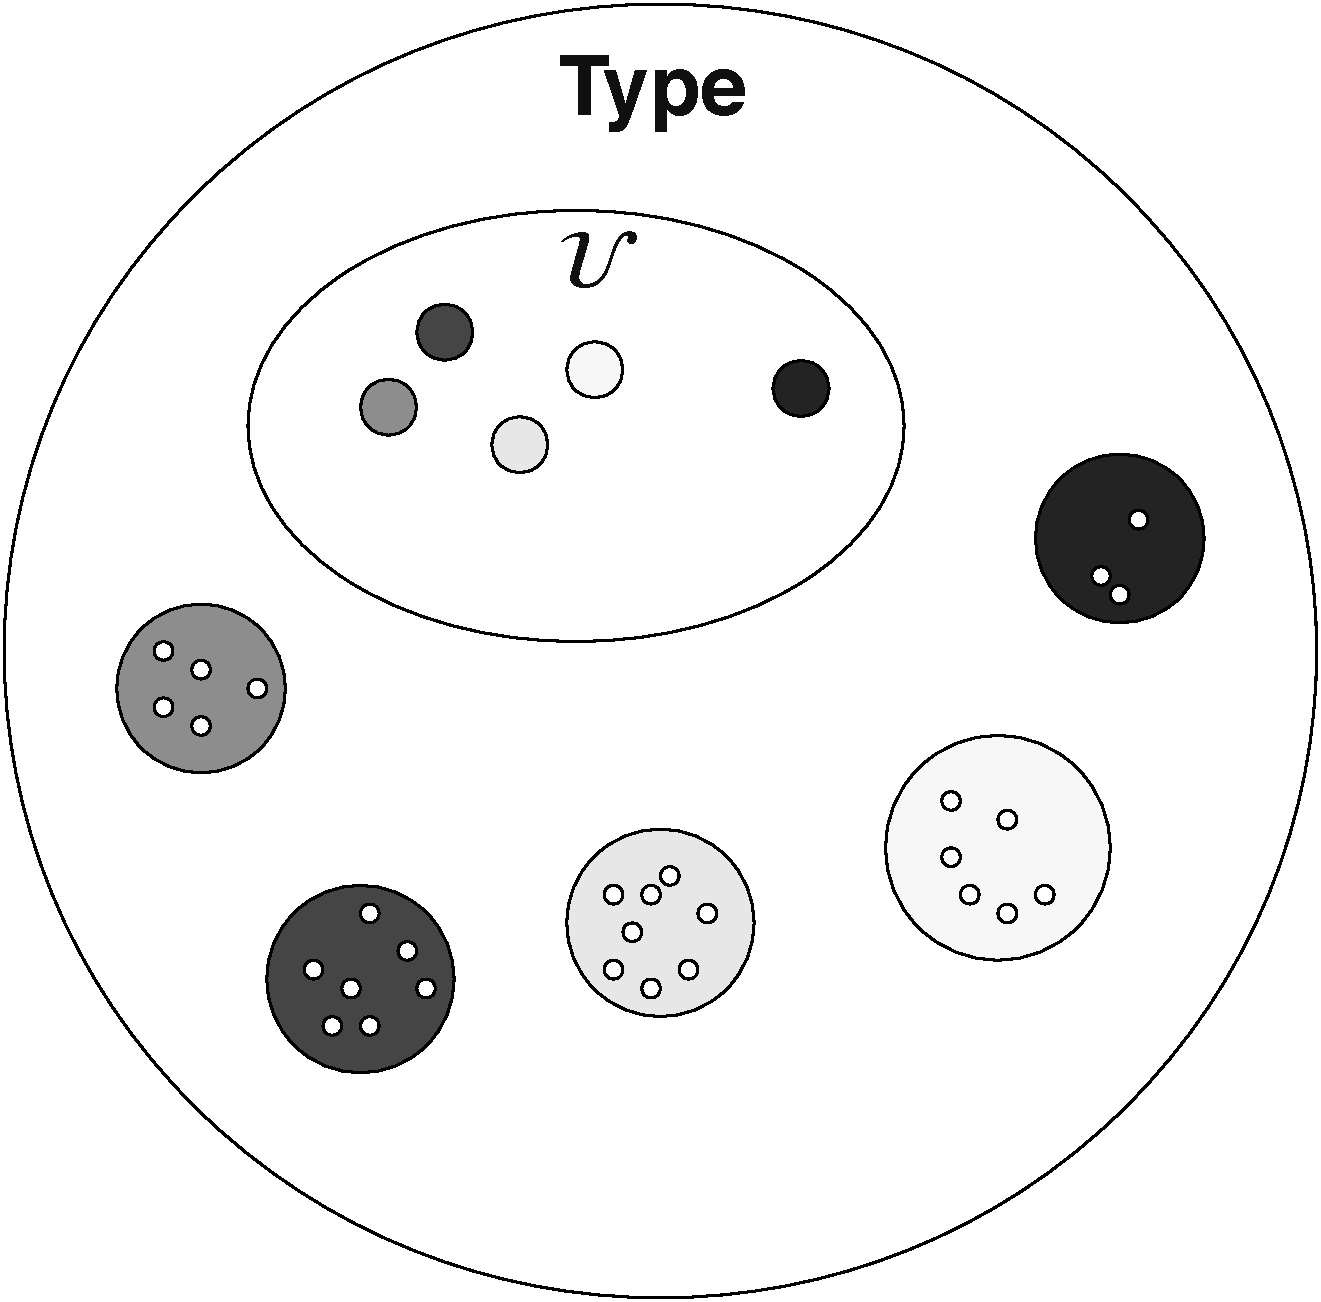
\includegraphics[width=2.8in]{universe-populated.pdf}
  \end{center}
\end{frame}

\begin{frame}
  \frametitle{Universes \`a la Tarski}
  \begin{center}
    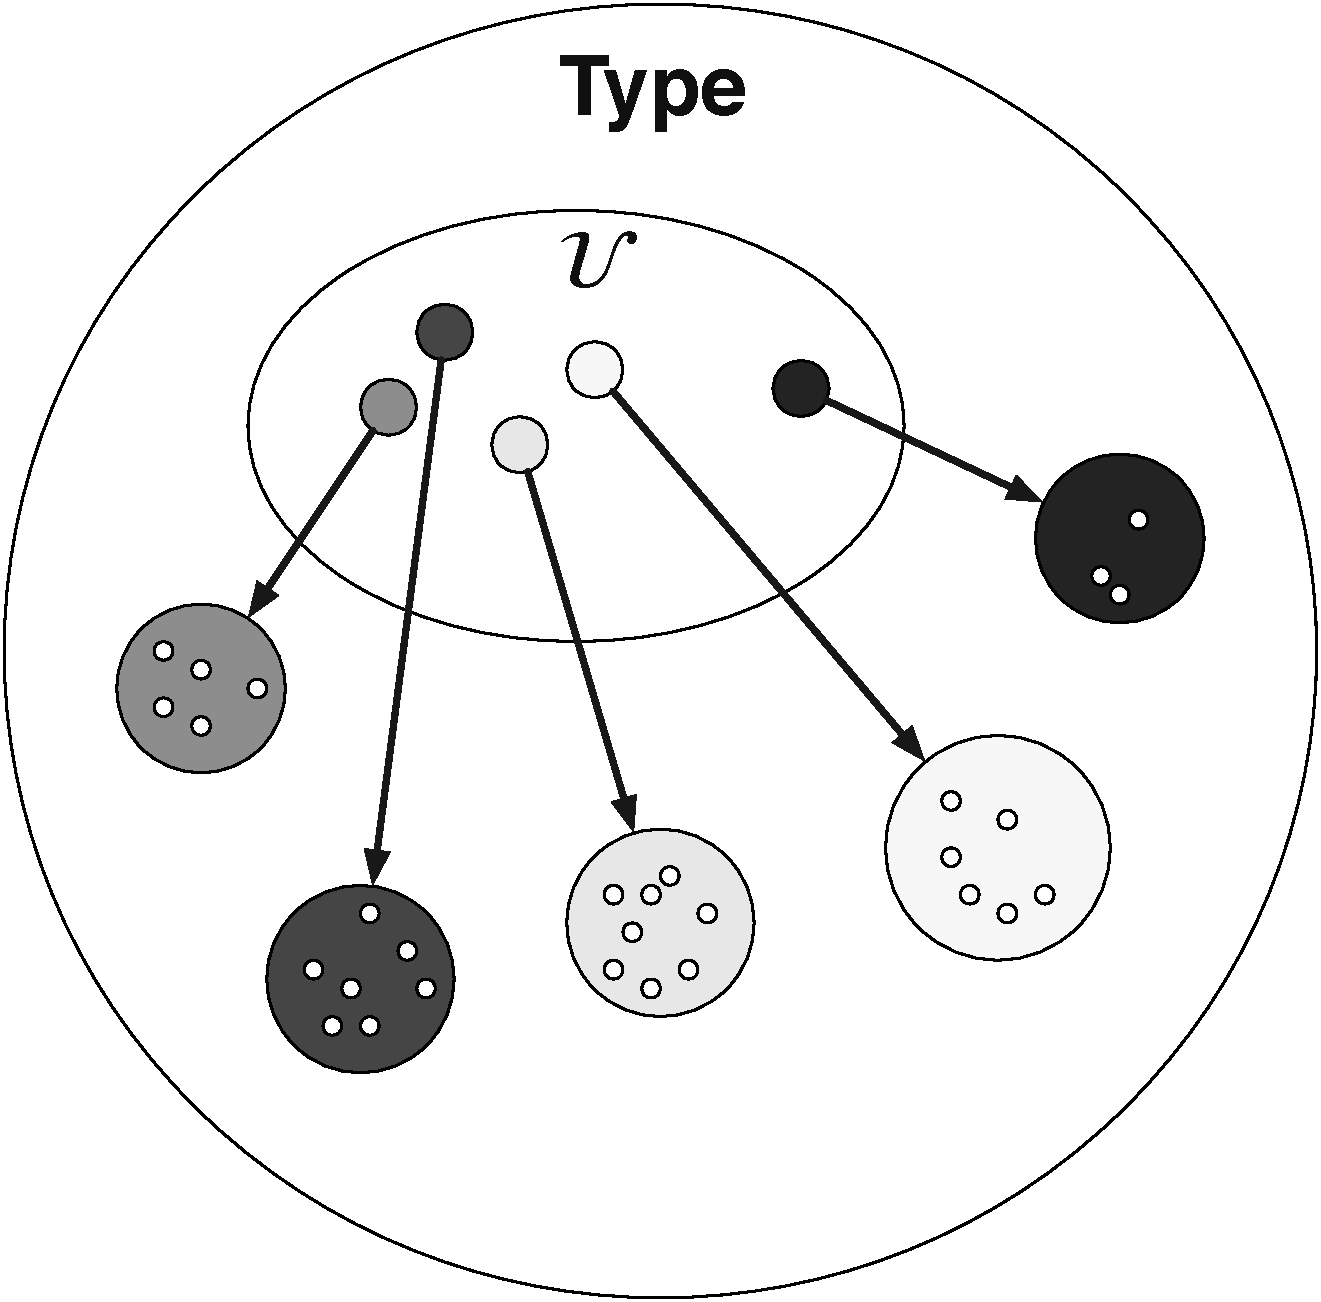
\includegraphics[width=2.8in]{universe-interpretation.pdf}
  \end{center}
\end{frame}

\begin{frame}
  \frametitle{A Closed Universe}
  \pause
  Let $\mathcal{A}$ be a universe of address books:
  \pause
  \begin{itemize}
    \item Statics:
      \pause
      \[
        \infer{\mathcal{A} : \Type}{}
        \qquad
        \pause
        \infer{\textsf{Label} : \Type}{}
        \qquad
        \pause
        \infer{\textit{Home}, \textit{Office} : \textsf{Label}}{}
      \]
      \pause
      \[
        \infer{\textsf{Name} : \mathcal{A}}{}
        \qquad
        \pause
        \infer{\textsf{Phone}[\ell],\textsf{Email}[\ell] : \mathcal{A}}{\ell : \textsf{Label}}
        \qquad
        \pause
        \infer{El_\mathcal{A}(s) : \Type}{s : \mathcal{A}}
      \]
      \pause
    \item Dynamics:
      \pause
      \[
        \infer{El_\mathcal{A}(\textsf{Name}) \leadsto \mathbf{string}}{}
        \qquad
        \pause
        \infer{El_\mathcal{A}(\textsf{Email}[\ell]) \leadsto \mathbf{string}}{}
      \]
      \pause
      \[
        \infer{El_\mathcal{A}(\textsf{Phone}[\ell]) \leadsto \mathsf{list}(\mathbb{N})}{}
      \]
  \end{itemize}
\end{frame}


\section{Type-Theoretic Records}

\begin{frame}
  \frametitle{Records as Products}
  \pause
  \only<2,3>{
    Records: the product of the image of $El_\mathcal{U}$ in $\Type$ restricted to a subset of $\mathcal{U}$.
  }
  \only<4>{
    \begin{center}
      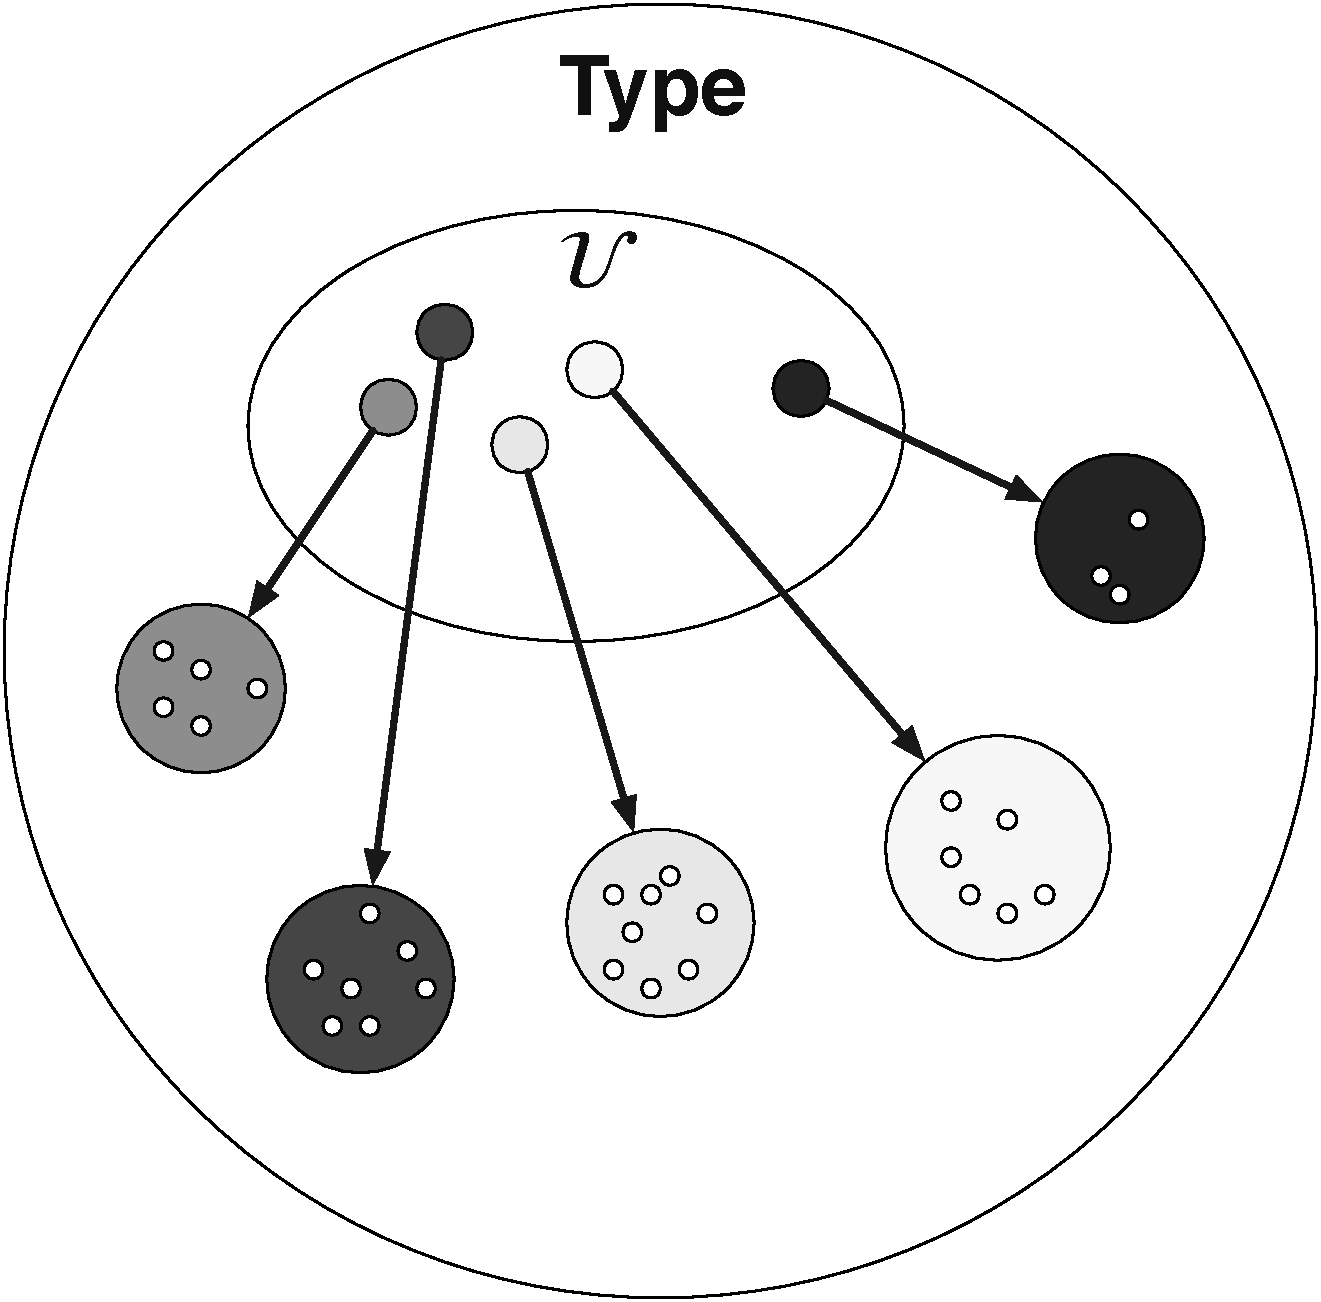
\includegraphics[width=2.8in]{universe-interpretation.pdf}
    \end{center}
  }
  \only<5>{
    \begin{center}
      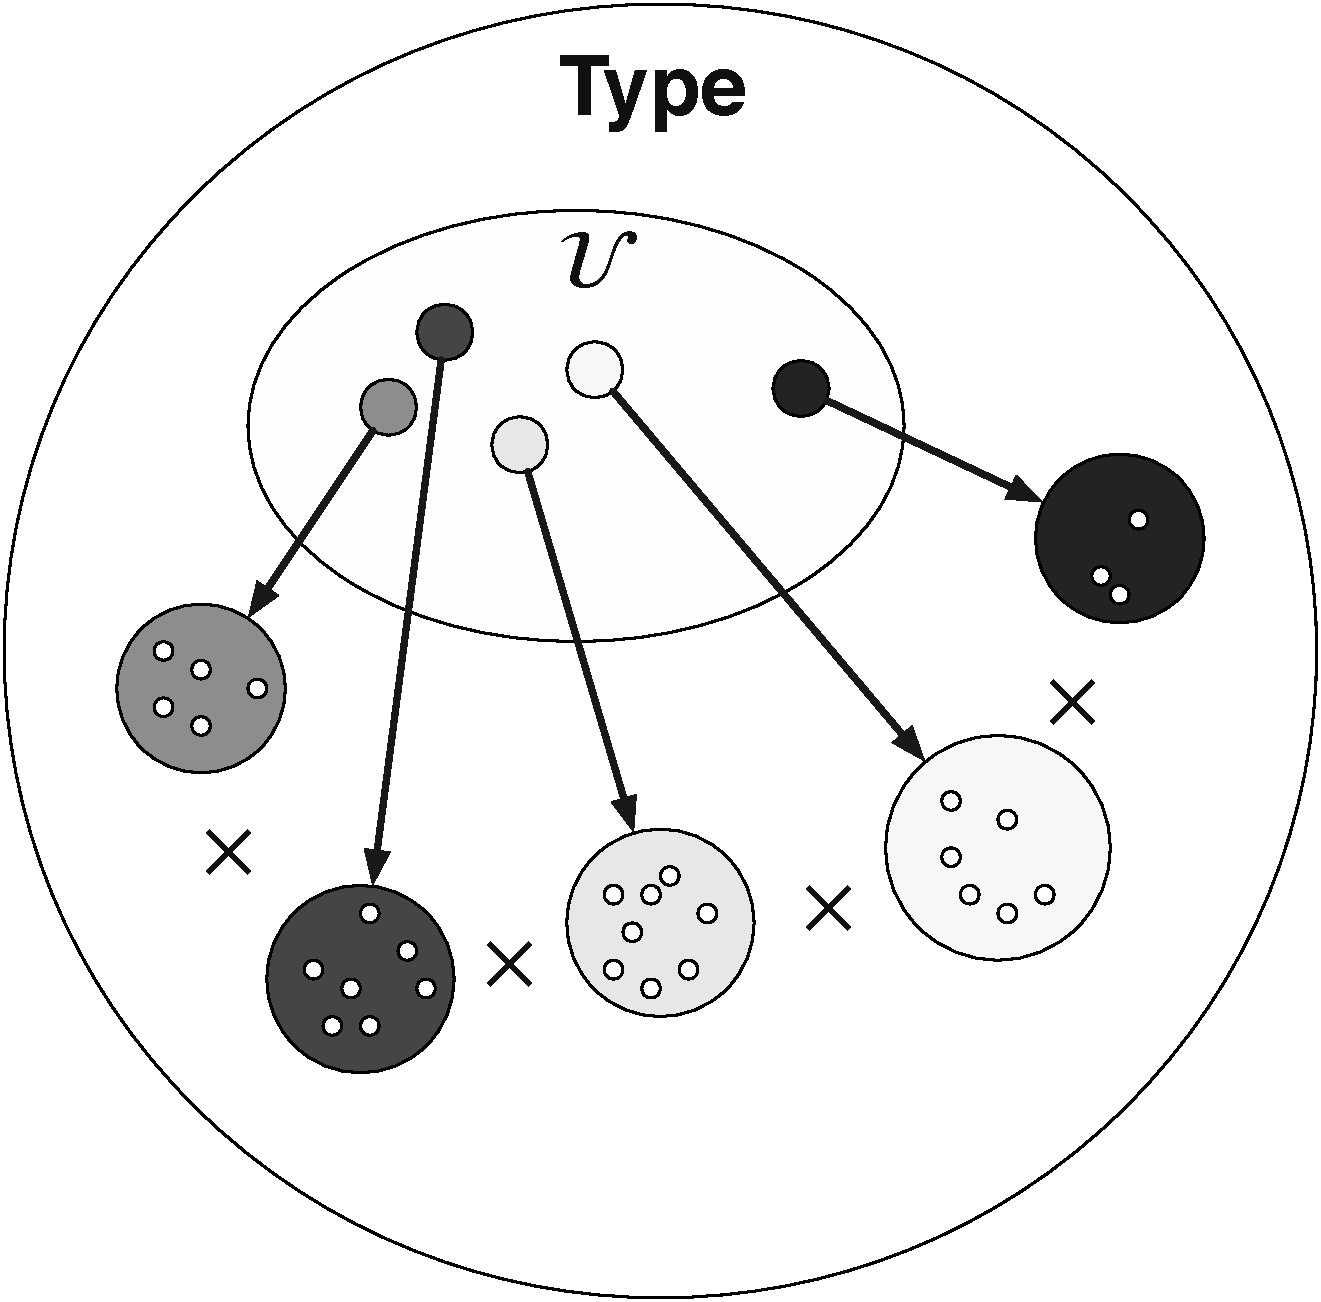
\includegraphics[width=2.8in]{universe-product.pdf}
    \end{center}
  }
  \only<3,6>{
    \[
      \mathsf{record}_\mathcal{U} \leadsto
        \sum_{\mathcal{V}\subset\mathcal{U}}
        \prod_\mathcal{V} El_\mathcal{U}|_\mathcal{V}
    \]
  }
\end{frame}

\begin{frame}
  \frametitle{Example Record}
  \[
    \begin{aligned}
      \mathsf{record}_\mathcal{U} &\leadsto
        \sum_{\mathcal{V}\subset\mathcal{U}}
        \prod_\mathcal{V} El_\mathcal{U}|_\mathcal{V}\\ \pause
      \mathcal{A}' &\leadsto \{ \mathsf{Name}, \mathsf{Email}\ \textit{Work} \}\\ \pause
      ex &: \mathsf{record}_\mathcal{U}\\ \pause
      ex &\leadsto \langle\mathcal{A}',\lambda.\\
         &\qquad \{\mathsf{Name}\mapsto \text{"Robert Harper"};\\
         &\qquad \ \mathsf{Email}\ \textit{Work}\mapsto \text{"rwh@cs.cmu.edu"} \}\rangle
    \end{aligned}
  \]
\end{frame}

\begin{frame}
  \frametitle{Corecords as Sums}
  \pause
  \only<2,3>{
    Corecords (extensible variants): the sum of the image of $El_\mathcal{U}$ in $\Type$ restricted to a subset of $\mathcal{U}$.
  }
  \only<4>{
    \begin{center}
      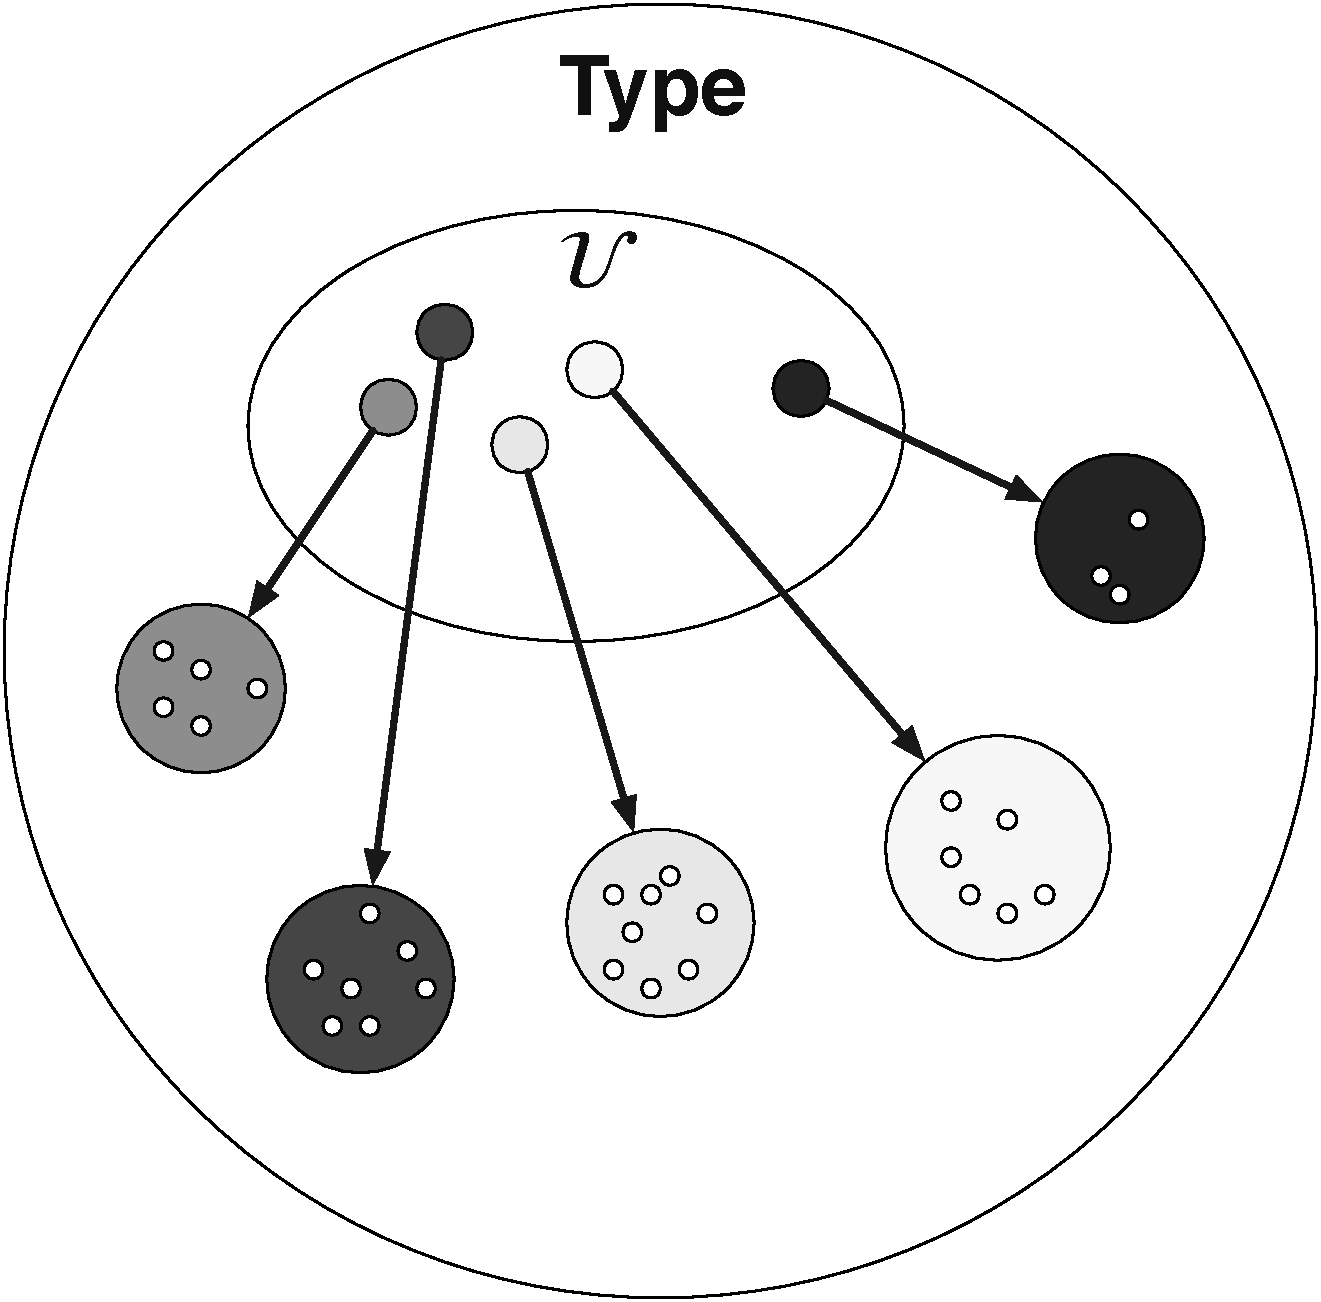
\includegraphics[width=2.8in]{universe-interpretation.pdf}
    \end{center}
  }
  \only<5>{
    \begin{center}
      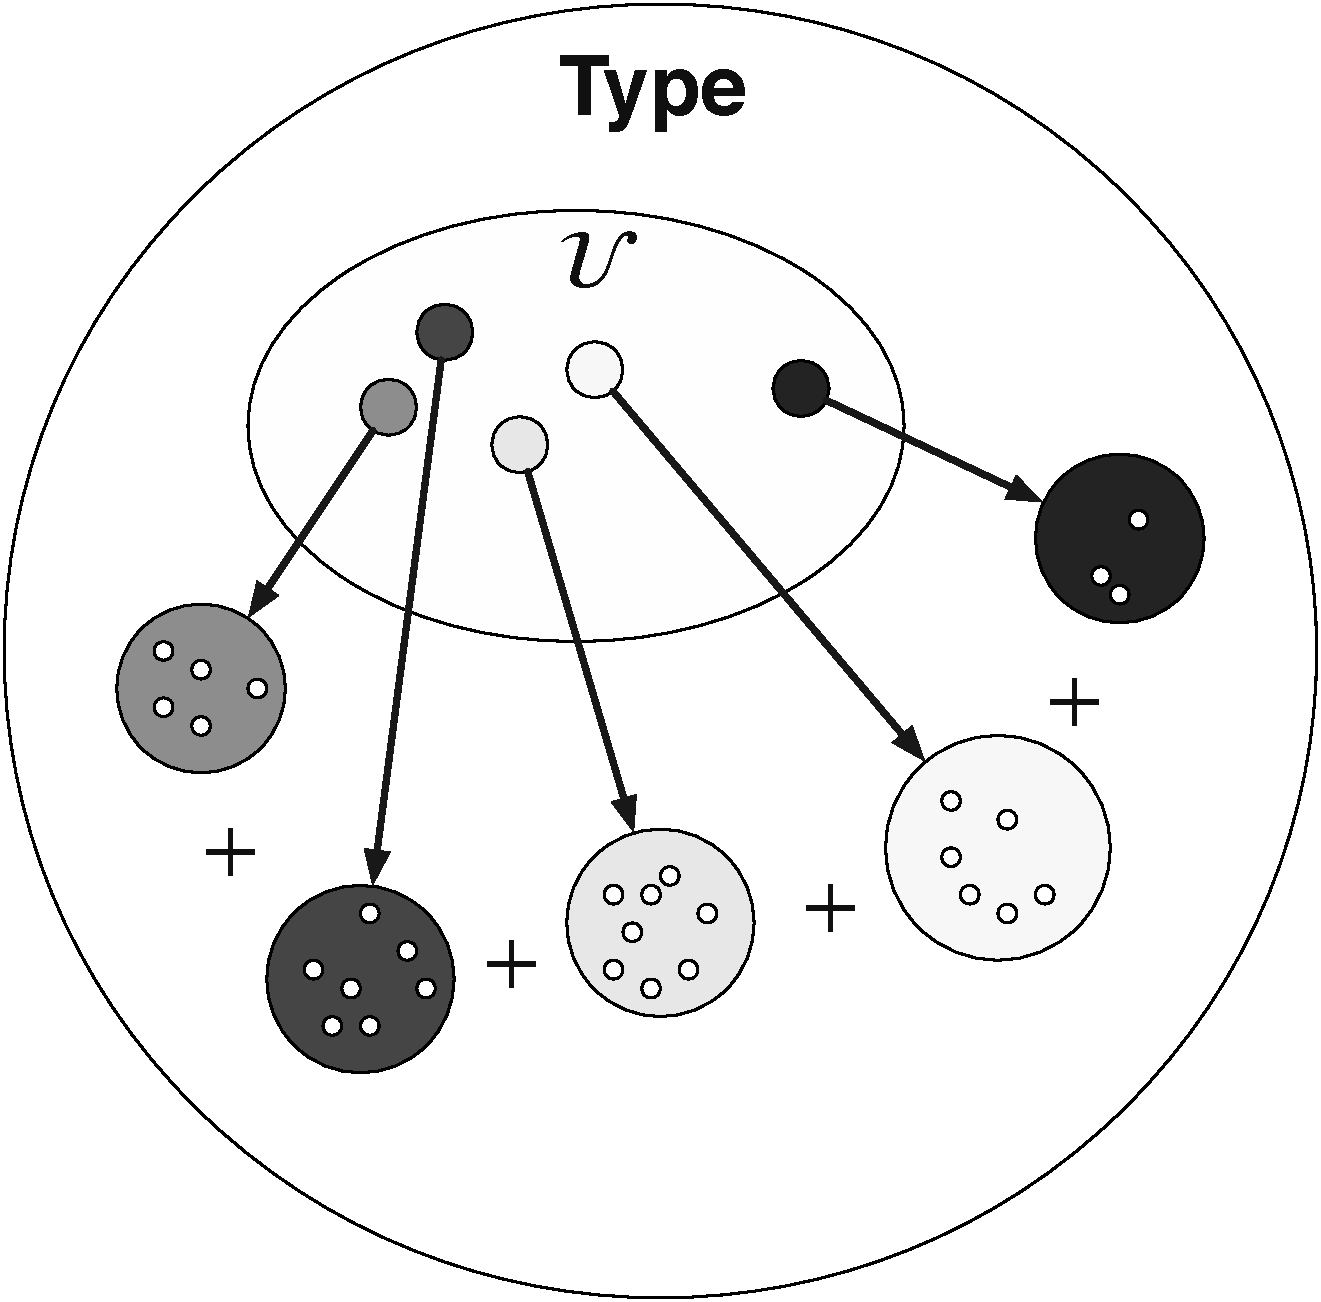
\includegraphics[width=2.8in]{universe-sum.pdf}
    \end{center}
  }
  \only<3,6>{
    \[
      \mathsf{corecord}_\mathcal{U} \leadsto
        \sum_{\mathcal{V}\subset\mathcal{U}}
        \sum_\mathcal{V} El_\mathcal{U}|_\mathcal{V}
    \]
  }
\end{frame}

\begin{frame}
  \frametitle{Doing it in Haskell}
  \pause
  \begin{itemize}
    \item Create a universe $\mathcal{U}$ at the type-level \pause
    \item Use type families to approximate $El_\mathcal{U}$ \pause
    \item Parameterize \lstinline{Rec} by $\mathcal{U}$, $El_\mathcal{U}$?
  \end{itemize}
\end{frame}

\begin{frame}[fragile]
  \frametitle{Records in Haskell}
  \begin{lstlisting}
  data Rec :: (|$\mathcal{U}$| -> *) -> [ |$\mathcal{U}$| ] -> * where |\pause|
    RNil :: Rec el|$_\mathcal{U}$| '[] |\pause|
    (:&) :: !(el|$_\mathcal{U}$| r) -> !(Rec el|$_\mathcal{U}$| rs) -> Rec el|$_\mathcal{U}$| (r ': rs)
  \end{lstlisting}
\end{frame}

\begin{frame}[fragile]
  \frametitle{Recovering HList}\pause
  \begin{lstlisting}
  type HList rs = Rec (|$\Lambda\tau.\;\tau$|) rs|\pause|

  ex :: HList [Int, Bool, String] |\pause|
  ex = 34 :& True :& "vinyl" :& RNil
  \end{lstlisting}
\end{frame}

\section{Effectful Records}

\begin{frame}[fragile]
  \frametitle{Validating Records}

  \begin{lstlisting}
  bob :: Rec El|$_\mathcal{A}$| [Name, Email Work] |\pause|
  bob = Name =: "Robert Harper"
      <+> Email Work =: "rwh@cs.cmu.edu"
  \end{lstlisting}
  \pause
  \begin{lstlisting}
  validateName :: String -> Either Error String
  validateEmail :: String -> Either Error String
  validatePhone :: [Nat] -> Either Error [Nat]
  \end{lstlisting}
  \pause
  \centerline{\textit{*unnnnnhhh...*}}
  \pause
  \begin{lstlisting}
  validateContact
    :: Rec El|$_\mathcal{A}$| [Name, Email Work]
    -> Either Error (Rec El|$_\mathcal{A}$| [Name, Email Work])
  \end{lstlisting}
\end{frame}
\begin{frame}
  \centerline{\textbf{Welp.}}
\end{frame}

\begin{frame}[fragile]
  \frametitle{Effects inside records}
  \begin{lstlisting}
  data Rec :: (|$\mathcal{U}$| -> *) -> [ |$\mathcal{U}$| ] -> * where
    RNil :: Rec el|$_\mathcal{U}$| '[]
    (:&) :: !(el|$_\mathcal{U}$| r) -> !(Rec el|$_\mathcal{U}$| rs) -> Rec el|$_\mathcal{U}$| (r ': rs)
  \end{lstlisting}
\end{frame}
\begin{frame}[fragile]
  \frametitle{Effects inside records}
  \begin{lstlisting}
  data Rec :: (|$\mathcal{U}$| -> *) -> (* -> *) -> [ |$\mathcal{U}$| ] -> * where
    RNil :: Rec el|$_\mathcal{U}$| f '[]
    (:&) :: !(f (el|$_\mathcal{U}$| r)) -> !(Rec el|$_\mathcal{U}$| f rs) -> Rec el|$_\mathcal{U}$| f (r ': rs)|\pause|

  (=:) : Applicative f => sing r -> el|$_\mathcal{U}$| r -> Rec el|$_\mathcal{U}$| f '[r]|\pause|
  k =: x = pure x :& RNil|\pause|

  (<-:) : sing r -> f (el|$_\mathcal{U}$| r) -> Rec el|$_\mathcal{U}$| f '[r]|\pause|
  k <-: x = x :& RNil
  \end{lstlisting}
\end{frame}

\begin{frame}[fragile]
  \frametitle{Compositional Validation}

  \begin{lstlisting}
  type Rec|$_\mathcal{A}$| = Rec El|$_\mathcal{A}$| |\pause|
  bob :: Rec|$_\mathcal{A}$| Identity [Name, Email Work] |\pause|
  bob = Name =: "Robert Harper"
      <+> Email Work =: "rwh@cs.cmu.edu"|\pause|
  \end{lstlisting}
\end{frame}

\begin{frame}[fragile]
  \frametitle{Compositional Validation}
  \begin{lstlisting}
  type Validator a = a -> Either Error a|\pause|
  validateName :: Rec|$_\mathcal{A}$| Validator '[Name]
  validatePhone :: forall |$\ell$|. Rec|$_\mathcal{A}$| Validator '[Phone |$\ell$|]
  validateEmail :: forall |$\ell$|. Rec|$_\mathcal{A}$| Validator '[Email |$\ell$|]|\pause|

  type TotalContact =
    [ Name, Email Home, Email Work
    , Phone Home, Phone Work ]|\pause|

  validateContact :: Rec|$_\mathcal{A}$| Validator TotalContact
  validateContact = validateName
                  <+> validateEmail
                  <+> validateEmail
                  <+> validatePhone
                  <+> validatePhone
  \end{lstlisting}
\end{frame}

\begin{frame}[fragile]
  \frametitle{Record Operators}\pause

  \begin{lstlisting}
  newtype Lift o f g x = Lift { runLift :: f x `o` g x }|\pause|

  type Validator = Lift (->) Identity (Either Error)|\pause|

  (<<*>>) :: Rec|$_\mathcal{U}$| (Lift (->) f g) rs -> Rec|$_\mathcal{U}$| f rs -> Rec|$_\mathcal{U}$| g rs|\pause|

  rdist :: Applicative f => Rec|$_\mathcal{U}$| f rs -> f (Rec|$_\mathcal{U}$| Identity rs)
  \end{lstlisting}
\end{frame}

\begin{frame}[fragile]
  \frametitle{Compositional Validation}

  \begin{lstlisting}
  newtype Lift o f g x = Lift { runLift :: f x `o` g x }
  type Validator = Lift (->) Identity (Either Error)
  (<<*>>) :: Rec|$_\mathcal{U}$| (Lift (->) f g) rs -> Rec|$_\mathcal{U}$| f rs -> Rec|$_\mathcal{U}$| g rs
  rdist :: Applicative f => Rec|$_\mathcal{U}$| f rs -> f (Rec|$_\mathcal{U}$| Identity rs)|\pause|

  validateContact :: Rec|$_\mathcal{A}$| Validator TotalContact|\pause|

  bobValid :: Rec|$_\mathcal{A}$| (Either Error) [Name, Email Work]|\pause|
  bobValid = cast validateContact <<*>> bob|\pause|

  validBob :: Either Error (Rec|$_\mathcal{A}$| Identity [Name, Email Work])|\pause|
  validBob = rdist bobValid
  \end{lstlisting}
\end{frame}

\begin{frame}
  \frametitle{Laziness as an effect}\pause

  \begin{itemize}
    \item Laziness considered harmful in the small\pause
    \item Vinyl records are strict in their constructors\pause
    \item Lazy variants usually accomplished through duplication\pause
    \item[$\uparrow$] \textbf{Utterly unacceptable}
  \end{itemize}
\end{frame}

\begin{frame}[fragile]
  \frametitle{Laziness as an effect}\pause

  \begin{lstlisting}
  newtype Identity a = Identity { runIdentity :: a }|\pause|
  data Thunk a = Thunk { unThunk :: a }|\pause|

  type PlainRec|$_\mathcal{U}$| rs = Rec|$_\mathcal{U}$| Identity rs|\pause|
  type LazyRec|$_\mathcal{U}$| rs = Rec|$_\mathcal{U}$| Thunk rs
  \end{lstlisting}
\end{frame}

\begin{frame}[fragile]
  \frametitle{Concurrent Records with Async}\pause

  \begin{lstlisting}
  fetchName :: Rec|$_\mathcal{A}$| IO '[Name]|\pause|
  fetchName = Name <-: someOperation|\pause|

  fetchWorkEmail :: Rec|$_\mathcal{A}$| IO '[Email Work]|\pause|
  fetchWorkEmail = Email Work <-: anotherOperation|\pause|

  fetchBob :: Rec|$_\mathcal{A}$| IO [Name, Email Work]|\pause|
  fetchBob = fetchName <+> fetchWorkEmail
  \end{lstlisting}
\end{frame}

\begin{frame}[fragile]
  \frametitle{Concurrent Records with Async}\pause

  \begin{lstlisting}
  newtype Concurrently a
    = Concurrently { runConcurrently :: IO a }|\pause|

  (<<map>>) :: (forall a. f a -> g a) -> Rec|$_\mathcal{U}$| f rs -> Rec|$_\mathcal{U}$| g rs|\pause|

  bobConcurrently :: Rec|$_\mathcal{A}$| Concurrently [Name, Email Work]|\pause|
  bobConcurrently = Concurrently <<map>> fetchBob|\pause|

  concurrentBob :: Concurrently (Rec|$_\mathcal{A}$| Identity [...])|\pause|
  concurrentBob = rdist bobConcurrently
  \end{lstlisting}
\end{frame}

\begin{frame}[fragile]
  \frametitle{Concurrent Records with Async}\pause

  \begin{lstlisting}
  fetchBob :: Rec|$_\mathcal{A}$| IO [Name, Email Work]
  bobConcurrently :: Rec|$_\mathcal{A}$| Concurrently [Name, Email Work]
  concurrentBob :: Concurrently (Rec|$_\mathcal{A}$| Identity [...])|\pause|

  bob :: IO (Rec|$_\mathcal{A}$| Identity [Name, Email Work])|\pause|
  bob = runConcurrently concurrentBob
  \end{lstlisting}
\end{frame}

\def\container{\mathsf{container}}
\newcommand\mkcon[2]{#1\triangleleft#2}

\begin{frame}
  \frametitle{Containers: The Syntax for Data Types}

  \[
    \infer{\container : \Type}{}\pause
    \qquad
    \infer{\mkcon{\mathcal{U}}{El_\mathcal{U}} : \container}{
      \mathcal{U} : \Type &
      El_\mathcal{U} : \mathcal{U} \to \Type
    }
  \]\pause
  \[
    \infer{C.\mathsf{Sh} : \Type}{C : \container}\pause
    \qquad
    \infer{C.\mathsf{Sh} \leadsto \mathcal{U}}{C \leadsto \mkcon{\mathcal{U}}{El_\mathcal{U}}}
  \]\pause
  \[
    \infer{C.\mathsf{Po} : C.\mathsf{Sh} \to \Type}{C : \container}\pause
    \qquad
    \infer{C.\mathsf{Po} \leadsto El_\mathcal{U}}{C \leadsto \mkcon{\mathcal{U}}{El_\mathcal{U}}}
  \]
\end{frame}

\begin{frame}
  \frametitle{Restricting Containers}
  \[
    \infer{C|_\mathcal{V} : \container}{
      C : \container &
      \mathcal{V} \subseteq C.\mathsf{Sh}
    }
  \]\pause
  \[
    \infer{
      C|_\mathcal{V}\leadsto \mkcon{\mathcal{V}}{El_\mathcal{U}|_\mathcal{V}}
    }{
      C \leadsto \mkcon{\mathcal{U}}{El_\mathcal{U}}
    }
  \]
\end{frame}
\begin{frame}
  \frametitle{Container Lifting}
  \[
    \infer{C\uparrow F : \container}{
      C : \container &
      F : \Type \to \Type
    }
  \]\pause
  \[
    \infer{
      \mkcon{C\uparrow F \leadsto \mathcal{U}}{F\circ El_\mathcal{U}}
    }{
      C \leadsto \mkcon{\mathcal{U}}{El_\mathcal{U}}
    }
  \]
\end{frame}

\begin{frame}
  \frametitle{A Menagerie of Quantifiers}\pause
  \only<2>{
    \emph{Dependent Products:}
    \[
      \infer{\Gamma\vdash\prod_AB : \Type}{
        \Gamma\vdash A: \Type &
        \Gamma, x:A \vdash B: \Type
      }
    \]
    \[
      \infer{\Gamma\vdash\lambda x. e : \prod_AB}{
        \Gamma,x:A\vdash e: B[x]
      }
    \]
  }
  \only<3>{
    \emph{Dependent Sums:}
    \[
      \infer{\Gamma\vdash\sum_AB : \Type}{
        \Gamma\vdash A: \Type &
        \Gamma, x:A \vdash B: \Type
      }
    \]
    \[
      \infer{\Gamma\vdash\langle a,b\rangle : \sum_AB}{
        \Gamma\vdash a:A &
        \Gamma\vdash b : B[a]
      }
    \]
  }
  \only<4>{
    \emph{Inductive Types:}
    \[
      \infer{\Gamma\vdash\Wtype_AB : \Type}{
        \Gamma\vdash A: \Type &
        \Gamma, x:A \vdash B: \Type
      }
    \]
    \[
      \infer{
        \Gamma\vdash\mathsf{sup}(a; v.\, b) : \Wtype_AB
      }{
        \Gamma\vdash a:A &
        \Gamma, v:B[a] \vdash b: \Wtype_AB
      }
    \]
  }
  \only<5>{
    \emph{Coinductive Types:}
    \[
      \infer{\Gamma\vdash\Mtype_AB : \Type}{
        \Gamma\vdash A: \Type &
        \Gamma, x:A \vdash B: \Type
      }
    \]
    \[
      \infer{
        \Gamma\vdash\mathsf{inf}(a; v.\, b) : \Mtype_AB
      }{
        \Gamma\vdash a:A &
        \Gamma, v:B[a] \vdash b: \infty\left(\Mtype_AB\right)
      }
    \]
  }
\end{frame}

\begin{frame}
  \frametitle{A Scheme for Quantifiers}
  \pause
  \[
    \infer{\Gamma\vdash Q\ \mathsf{quantifier}}{
      \Gamma,A:\Type, (x:A\vdash B:\Type) \vdash Q_AB:\Type
    }
  \]
\end{frame}

\begin{frame}
  \frametitle{Quantifiers Give Containers Semantics}
  \[
    \infer{\Gamma\vdash Q\ \mathsf{quantifier}}{
      \Gamma,A:\Type, (x:A\vdash B:\Type) \vdash Q_AB:\Type
    }
  \]\pause
  \[
    \infer{\llbracket C\rrbracket_Q : \Type}{
      C : \container &
      Q\ \mathsf{quantifier}
    }
  \]\pause
  \[
    \infer{
      \llbracket C\rrbracket_Q \leadsto Q_\mathcal{U} El_\mathcal{U}
    }{
      C \leadsto \mkcon{\mathcal{U}}{El_\mathcal{U}}
    }
  \]
\end{frame}

\begin{frame}
  \frametitle{Vinyl Records as Containers}\pause
  Records and corecords are finite products and sums respectively.\pause
  \[
    \begin{aligned}
      \mathsf{Rec}\ El_\mathcal{U}\ F\ rs
        &\cong \left\llbracket (\mkcon{\mathcal{U}}{El_\mathcal{U}})|_{rs\ni-}\uparrow F \right\rrbracket_\Pi\\ \pause
      \mathsf{CoRec}\ El_\mathcal{U}\ F\ rs
        &\cong \left\llbracket (\mkcon{\mathcal{U}}{El_\mathcal{U}})|_{rs\ni-}\uparrow F \right\rrbracket_\Sigma\\ \pause
      \\
      ???\ El_\mathcal{U}\ F\ rs
        &\cong \left\llbracket (\mkcon{\mathcal{U}}{El_\mathcal{U}})|_{rs\ni-}\uparrow F \right\rrbracket_\mathrm{W}\\ \pause
      ???\ El_\mathcal{U}\ F\ rs
        &\cong \left\llbracket (\mkcon{\mathcal{U}}{El_\mathcal{U}})|_{rs\ni-}\uparrow F \right\rrbracket_\mathrm{M}
    \end{aligned}
  \]
\end{frame}

\begin{frame}
  \centerline{\textbf{Questions}}
\end{frame}

\end{document}

